\documentclass[journal,12pt,twocolumn]{IEEEtran}
\usepackage[utf8]{inputenc}
\usepackage{amsmath}
\usepackage{graphicx}
\usepackage[export]{adjustbox}
\usepackage[usenames, dvipsnames]{color}
\renewcommand\lstlistingname{}
 \lstset{
	language=vhdl,
	basicstyle=\small\sffamily,
	tabsize=3,
	numbers=left,
	numberstyle=\tiny,
	frame=tb,
	keepspaces,
	commentstyle=\color{green},
	keywordstyle=\color{red}
} 

\title{I2C}
\begin{document}
	\maketitle

	% topics to write - disadvantage of SPI, I2C protocol, our way of implementation
	\paragraph{Introduction}
		The Inter-Integrated Circuit (I2C) protocol is intended to allow multiple slave digital integrated chips (circuits) to comunicate with one or more master chips. It is a 2-wire, bidirectional data link invented and specified by Philips. The two lines of the I2C bus are SDA and SCL. SCL is a serial clock line and SCA is a serial data line. 

		

	\begin{figure}[h!] % [h] - here (same location) and ! is for override
		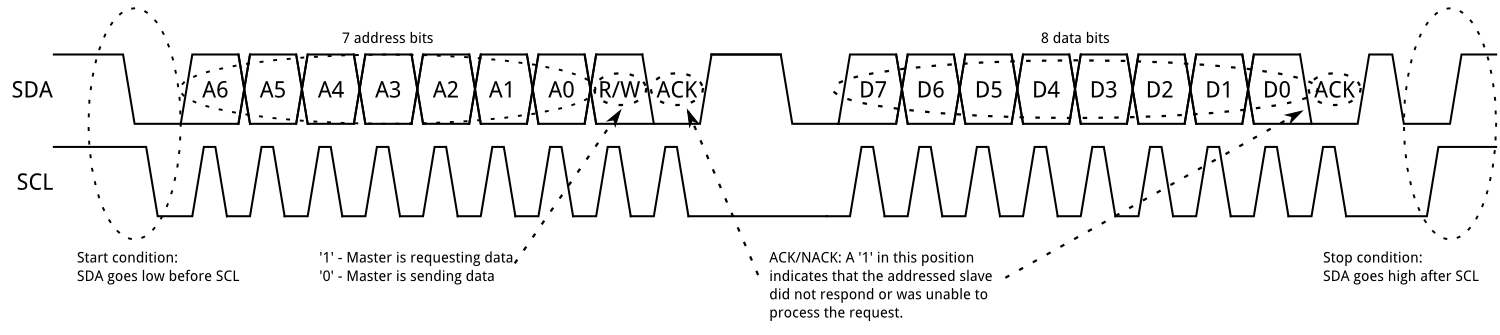
\includegraphics[width=\linnewidth]{i2c_concept.png}
		\label{fig: I2C protocol}
	\end{figure}

	\begin{figure}[p] % [p] is to put the image in an extra page
		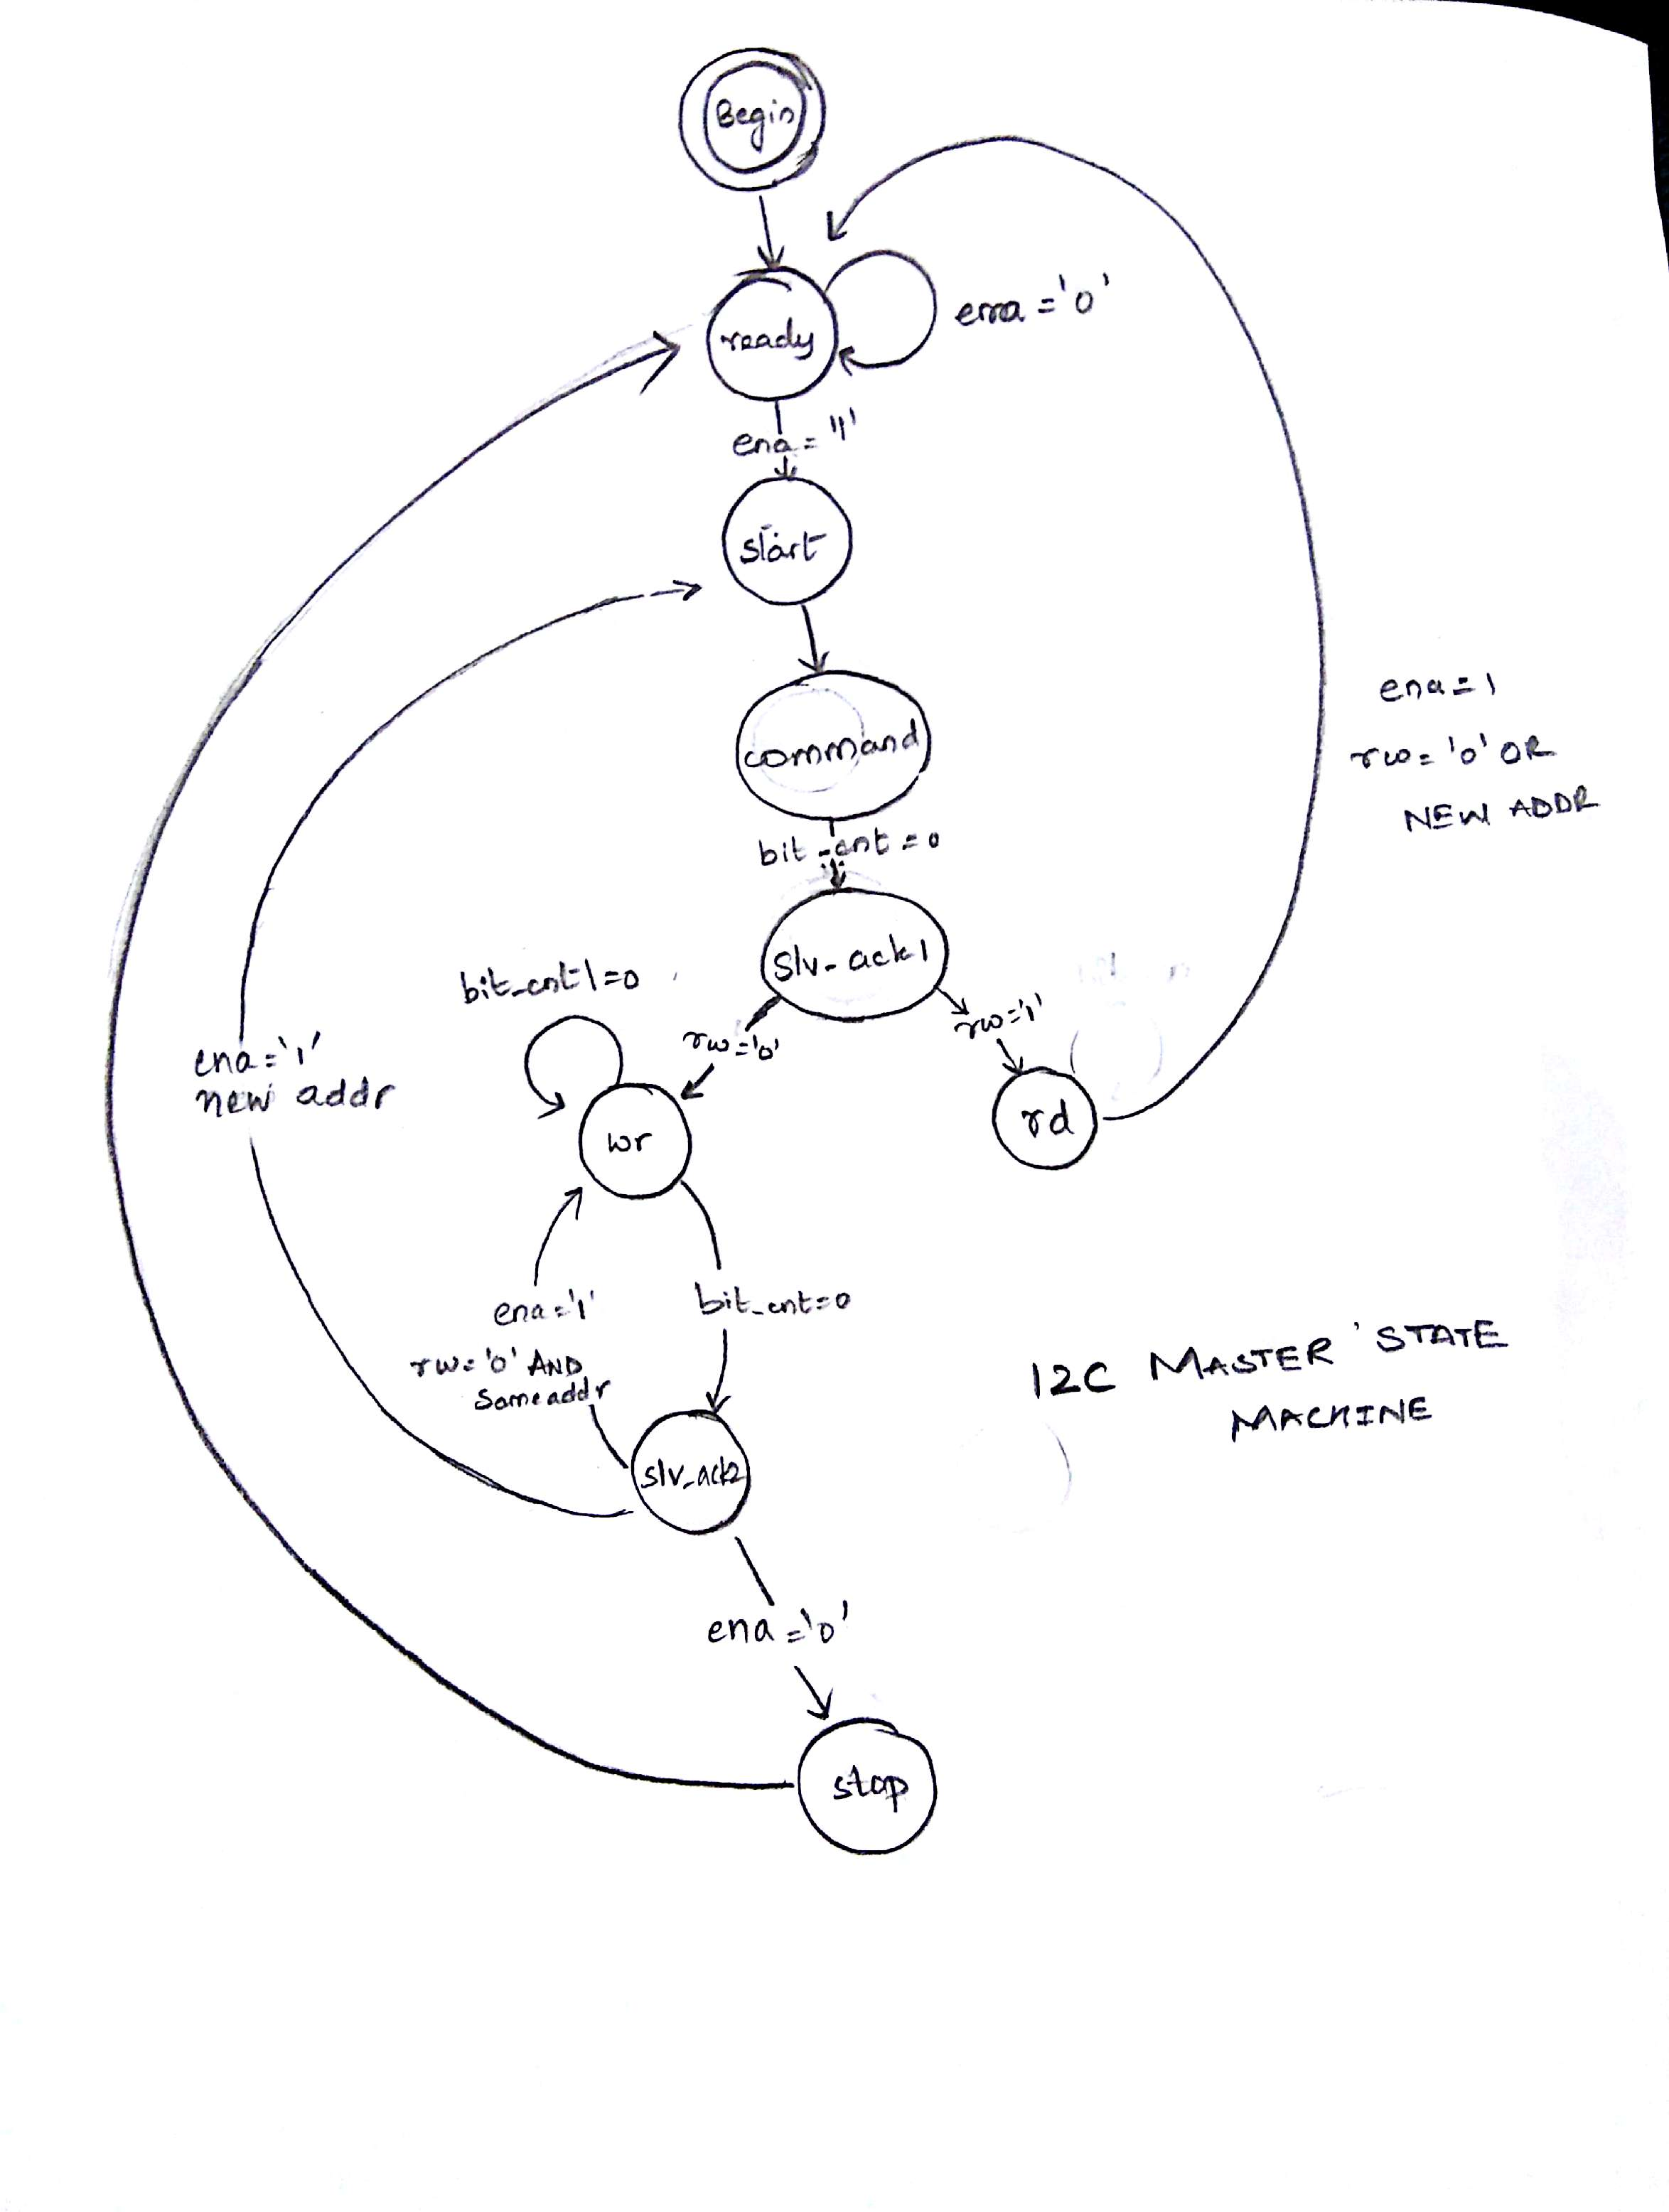
\includegraphics[width=\linewidth]{i2c_state_diagram.JPG}
	\end{figure}


	\begin{lstlisting}
		%code snippets here
		code here. 
	\end{lstlisting}

\end{document}

